% ============================================================
%  SECTION 1 — INTRODUCTION
% ============================================================% ------------------------------------------------------------
\subsection{Motivation and Problem Context}
\label{subsec:motivation}
% ------------------------------------------------------------

Large infrastructure and engineering projects routinely overrun their budgets
and miss their schedules. Across a database of thousands of projects spanning
seven decades, \citet{Flyvbjerg2003} document that cost overruns are the norm
rather than the exception, with mean overruns exceeding 20\% in transportation
infrastructure and reaching 70\% in large-scale IT systems.
\citet{Merrow2011} reports that fewer than 40\% of industrial megaprojects
achieve their approved cost and schedule targets. These figures describe
individual projects. When a portfolio of such projects is executed
simultaneously under a single governing body and a shared capital commitment,
the risks compound: a cash-flow shortfall on one project propagates immediately
to others, and the decision of how much budget to direct to each project at
each period can determine whether the portfolio as a whole succeeds or fails.

Despite this, the formal treatment of the portfolio-level budget allocation
problem as a sequential decision-making problem is conspicuously absent from
the project portfolio management literature. Research attention has been
concentrated at the \emph{selection} stage --- which projects to include in the
portfolio --- while the \emph{operational governance} stage --- how to manage
the portfolio of committed projects through to completion --- has received
comparatively little analytical treatment
\citep{Archer1999, Cooper2001, Turner2014}. The present work fills this gap.

We consider a portfolio of $n$ projects, each governed by a bilateral contract
consistent with FIDIC forms \citep{FIDIC2017}, executing concurrently under a
fixed capital commitment. A portfolio manager --- a board, investment committee,
or programme director --- exercises a single recurring decision at each discrete
planning period: how much budget to allocate to each active project. All
strategic and operational outcomes of interest flow through this allocation
decision. The formal problem is to find the allocation policy that maximises
discounted net cash flow across the portfolio horizon while satisfying hard
liquidity constraints, respecting contract mechanics.

% ------------------------------------------------------------
\subsection{The Project Management Decision Hierarchy}
\label{subsec:hierarchy}
% ------------------------------------------------------------

To situate the present contribution precisely, it is useful to distinguish the
three nested decision layers that constitute project portfolio management
\citep{PMI2017}.

\paragraph{Portfolio selection.}
The selection problem asks: given a candidate set of projects and a capital
budget, which subset should the organisation commit to? This is a combinatorial
optimisation problem studied extensively in the literature using mean-variance
portfolio theory \citep{Markowitz1952, Eilat2006}, multi-criteria decision
analysis \citep{Martinsuo2007}, and metaheuristic methods \citep{Zhang2020}.
The present work treats selection as an exogenous input: the portfolio of
committed projects is fixed at the start of the planning horizon, and contracts
have already been signed. This decomposition is consistent with the two-stage
governance model of \citet{Turner2014} and the PMI Standard for Portfolio
Management \citep{PMI2017}.

\paragraph{Portfolio governance.}
Once a portfolio is committed, the governing body must monitor and control
execution. This is the layer at which the present work operates. The governing
body does not manage individual projects directly --- that is the contractor's
role --- but it controls the budget directed to each project at each period.
This single continuous allocation decision is the sole instrument of the
portfolio manager. Termination is not a discrete agent action but an endogenous environment
mechanic demonstrating project failure; it is preceded by a cure period modelled
as a project-specific tolerance counter observable in the portfolio state.

\begin{figure}[htbp]
\centering
\begin{tikzpicture}[
    node distance=1.8cm,
    box/.style={rectangle, rounded corners=5pt, draw=black!60,
                fill=blue!8, minimum width=4.2cm,
                minimum height=1.2cm, align=center, font=\small},
    env/.style={rectangle, rounded corners=5pt, draw=black!60,
                fill=orange!10, minimum width=4.2cm,
                minimum height=1.2cm, align=center, font=\small},
    obs/.style={rectangle, rounded corners=5pt, draw=black!60,
                fill=green!8, minimum width=10.2cm,
                minimum height=1.4cm, align=center, font=\small},
    arr/.style={->, thick},
    ]

    \node[box] (pm)
    {\textbf{Portfolio Manager}\\policy $\pi(S_t) \to \mathbf{x}_t$};

    \node[env, right=3.8cm of pm] (contractor)
    {\textbf{Contractor}\\project execution};

    \node[obs, below=2.4cm of $(pm)!0.5!(contractor)$] (state)
    {\textbf{Observable State} $S_t$:\quad
        $\bigl\{P_{i,t}^{\mathrm{actual}},\;
        \mathrm{CPI}_{i,t},\;\mathrm{SPI}_{i,t},\;
        \delta_{i,t},\;\Delta_{i,t}^{\mathrm{pen}},\;
        \mathrm{status}_{i,t},\;\tau_{i,t}^{\mathrm{rem}}\bigr\}_{i},\;B_t$};

    \draw[arr, blue!60!black] (pm.east) -- (contractor.west)
    node[midway, above, font=\footnotesize] {allocation $\mathbf{x}_t$};

    \draw[arr, orange!70!black]
    (contractor.south) -- ++(0,-0.85) -| (state.north east)
    node[near start, right, font=\footnotesize, align=left]
        {$\Delta P_{i,t} = \eta_{i,t}\,x_{i,t}/\mathrm{BAC}_i$\\
        \textcolor{gray!70}{($\eta_{i,t}$ unobservable)}};

    \draw[arr, green!50!black]
    (state.north west) -- ++(0,0.85) -| (pm.south)
    node[near start, left, font=\footnotesize] {observe $S_t$};

    \draw[arr, dashed, green!55!black]
    (contractor.north) -- ++(0,1.1)
    -- ++(-6.0,0)
    -- (pm.north)
    node[near end, above, font=\footnotesize, green!55!black, xshift=1.2cm]
        {FIDIC payments:\;
        $R_{i,j}^{\mathrm{net}},\;R_i^{\mathrm{ret}},\;R_i^{\mathrm{term}}$};

\end{tikzpicture}
\caption{Portfolio governance feedback loop. The portfolio manager (agent)
    controls only the budget allocation vector $\mathbf{x}_t$. Contractors
    convert allocations into physical progress through efficiency $\eta_{i,t}$,
    which is unobservable and realized only after commitment. The full state
    $S_t$ is observable each period; FIDIC milestone payments, retention
    release, and termination settlement flow back as cash inflows.}
\label{fig:feedback_loop}
\end{figure}

\paragraph{Project execution.}
At the project level, the contractor controls workforce, materials, equipment,
and subcontracting. The portfolio manager observes the outcomes of these
decisions --- cumulative progress, earned value, payment certifications ---
but does not control them. The efficiency with which a budget allocation is
converted into physical progress is determined at the project level and is
uncertain from the portfolio manager's perspective.

This hierarchy is central to the modelling architecture: the formulation
developed in Section~\ref{sec:problem_formulation} lives entirely at the
portfolio governance layer, with project execution dynamics appearing only as
parameters (deterministic at Level~1, stochastic at Levels~2 and~3).

% ------------------------------------------------------------
\subsection{Contract Mechanics and Cash-Flow Structure}
\label{subsec:contract_mechanics}
% ------------------------------------------------------------

The financial interaction between the portfolio manager (as client) and each
contractor is governed by the contract. This paper parameterises all contract
mechanics consistently with FIDIC Red, Yellow, and Silver Book forms
\citep{FIDIC2017}, which represent the dominant international framework for
EPC contracting. Understanding the cash-flow structure is essential to
understanding the optimisation problem; this subsection provides that
foundation.

\paragraph{Milestone-based payment.}
Rather than paying contractors on a time-basis, FIDIC contracts structure
payment around certified milestones: discrete progress thresholds at which the
client verifies that a specified scope fraction has been physically completed
and releases the corresponding payment. The gross payment at milestone $j$ is a
contractually fixed fraction $\phi_{i,j}$ of the contract price $CP_i$.
Because payment is contingent on certified progress, the timing of cash
inflows is a function of the contractor's actual performance and, through the
portfolio manager's allocation decisions, of the budget directed to the project.
This creates the fundamental linkage between allocation decisions and cash
inflows that makes the problem non-trivial.

\paragraph{Advance payment and progressive recovery.}
At project initiation, the client disburses an advance payment $A_i =
\alpha_i \cdot CP_i$ to the contractor. This is a timing instrument: it
reduces the contractor's early working-capital burden and is recovered
progressively through percentage deductions from subsequent interim payment
certificates, with the deduction rate $\delta_i^{\mathrm{rec}}$ and
commencement threshold $\psi_i$ specified as project-specific contract
parameters \citep{FIDIC2017}. The advance payment creates an immediate cash inflow at project start and a
series of reduced inflows at each certified milestone, both of which must be
tracked in the portfolio cash balance. Interim milestone payments are
additionally subject to stochastic timing delays between certification and
receipt, consistent with observed payment practices in international EPC
contracting \citep{Aibinu2006, Odeh2002}; the amount transferred equals the
contractually fixed net milestone value, but the period of receipt is a random
variable.

\paragraph{Retention.}
A fraction $\rho_i$ of each milestone payment is withheld by the client as a
performance bond. The accumulated retention $R_i^{\mathrm{ret}} = \rho_i
\cdot CP_i$ is released in full upon project completion. Retention creates a
structural completion incentive embedded in the payment mechanics: the larger
the retention fraction, the more strongly the cash flow profile rewards
completion over partial delivery. In the formulation, retention release enters
the portfolio cash balance as a lump inflow in the period the final milestone
is certified.

\paragraph{Earned value management as a performance signal.}
The Earned Value Management framework \citep{Fleming2010} provides the
diagnostic vocabulary used to monitor contractor performance. The Cost
Performance Index $\mathrm{CPI}_{i,t} = \text{BCWP}_{i,t} /
\text{ACWP}_{i,t}$ measures how much budgeted value has been earned per unit
of actual expenditure; values below unity indicate cost overrun. The Schedule
Performance Index $\mathrm{SPI}_{i,t} = \text{BCWP}_{i,t} /
\text{BCWS}_{i,t}$ measures actual progress relative to planned progress;
values below unity indicate schedule lag \citep{Fleming2010}. In the present
formulation, these indices are observable state variables that inform the
allocation decision; their stochastic dynamics at Levels~2 and~3 are
calibrated from empirical EVM datasets \citep{Acebes2015, Batselier2017}.

\paragraph{S-curve expenditure profiles.}
The planned expenditure of a construction or engineering project follows a
characteristic sigmoid profile over its planned duration: slow ramp-up in the
mobilisation phase, rapid expenditure in the peak execution phase, and tapering
in the close-out phase \citep{Kenley2009}. This profile is modelled using the
regularized incomplete Beta function $F_i(\tau) = I_\tau(a_i, b_i)$, whose
shape parameters $(a_i, b_i)$ are calibrated from project data. The planned
cumulative expenditure fraction at normalised time $\tau_{i,t}$ provides the
baseline against which actual progress is measured throughout the formulation.

\paragraph{Termination.}
FIDIC contracts provide for client-initiated termination when the contractor
has materially breached the contract --- most commonly through sustained failure
to meet schedule obligations. Termination triggers a settlement payment based
on the value of work completed at the termination date, net of any outstanding
advance recovery obligation. In the present model, termination is an endogenous environment mechanic, not a
deliberate agent action. It is triggered when two conditions hold simultaneously
for a project-specific number of consecutive periods --- the termination
tolerance $\tau_i^{\mathrm{tol}}$: the forecast finish deviation has exceeded
the contractual penalty ceiling, and the cost performance index has fallen below
a project-specific recovery threshold $\kappa_i$. This joint persistence
requirement models the FIDIC cure period \citep{FIDIC2017, Ndekugri2008}, the
contractually prescribed interval during which both parties are obliged to
attempt performance recovery before the client may formally terminate. The
tolerance counter $\tau_{i,t}^{\mathrm{rem}}$ --- periods remaining before
termination executes --- is part of the observable environment state; the agent
cannot override its dynamics but observes its value and can influence it
indirectly through allocation decisions that affect $\mathrm{SPI}_{i,t}$ and
$\mathrm{CPI}_{i,t}$. When the counter reaches zero, termination executes in
the following period, and its timing affects the portfolio cash balance through
the settlement payment $R_i^{\mathrm{term}}$, which may be positive or negative
depending on the advance recovery position.

\begin{figure}[htbp]
\centering
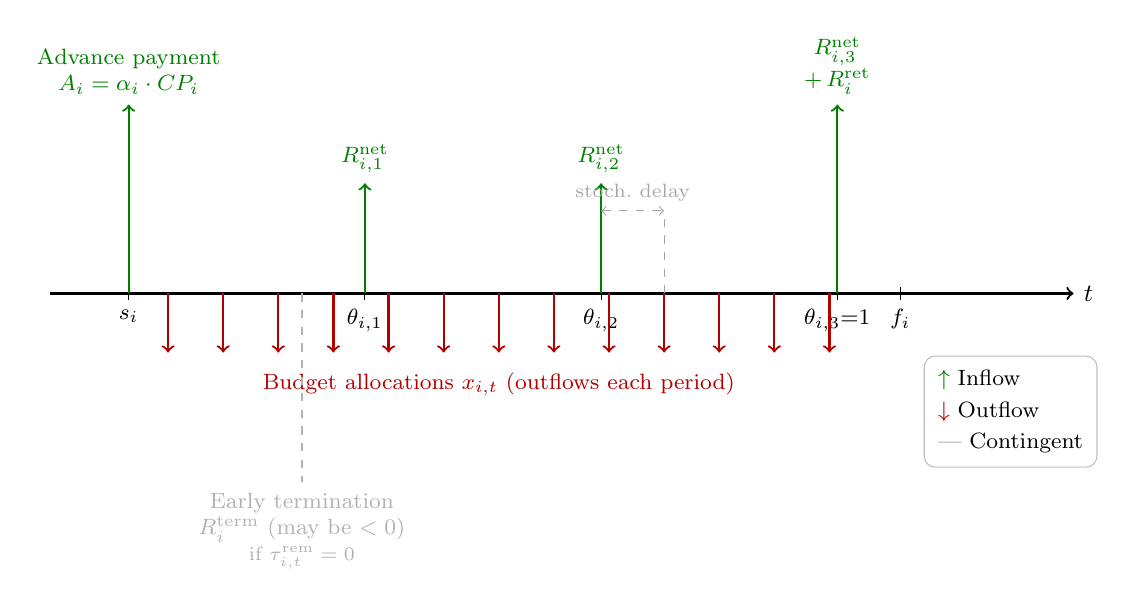
\begin{tikzpicture}[
    every node/.style={font=\small},
    inflow/.style={->, thick, green!50!black},
    outflow/.style={->, thick, red!70!black},
    ]

    \draw[->, thick] (0,0) -- (13.0,0) node[right] {$t$};

    \foreach \x/\lbl in {1/$s_i$, 4/$\theta_{i,1}$, 7/$\theta_{i,2}$,
                        10/$\theta_{i,3}{=}1$, 10.8/$f_i$}{
    \draw (\x,0.08) -- (\x,-0.08)
        node[below, font=\footnotesize] {\lbl};
    }

    \draw[inflow] (1,0) -- (1,2.4)
    node[above, align=center, font=\footnotesize]
        {Advance payment\\$A_i = \alpha_i \cdot CP_i$};

    \draw[inflow] (4,0) -- (4,1.4)
    node[above, font=\footnotesize] {$R_{i,1}^{\mathrm{net}}$};
    \draw[inflow] (7,0) -- (7,1.4)
    node[above, font=\footnotesize] {$R_{i,2}^{\mathrm{net}}$};

    \draw[<->, dashed, gray!70] (7,1.05) -- (7.8,1.05)
    node[midway, above, font=\scriptsize, gray!70] {stoch.\ delay};
    \draw[dashed, gray!70] (7.8,0) -- (7.8,1.05);

    \draw[inflow] (10,0) -- (10,2.4)
    node[above, align=center, font=\footnotesize]
        {$R_{i,3}^{\mathrm{net}}$\\$+\,R_i^{\mathrm{ret}}$};

    \foreach \x in {1.5,2.2,2.9,3.6,4.3,5.0,5.7,6.4,7.1,7.8,8.5,9.2,9.9}{
    \draw[outflow] (\x,0) -- (\x,-0.75);
    }
    \node[red!70!black, font=\footnotesize]
    at (5.7,-1.15) {Budget allocations $x_{i,t}$ (outflows each period)};

    \draw[dashed, thick, gray!60] (3.2,0) -- (3.2,-2.4)
    node[below, align=center, font=\footnotesize, gray!60]
        {Early termination\\$R_i^{\mathrm{term}}$ (may be $<0$)\\
        {\scriptsize if $\tau_{i,t}^{\mathrm{rem}}=0$}};

    \node[draw=gray!50, rounded corners, inner sep=5pt,
        align=left, font=\footnotesize] at (12.2,-1.5) {
    \textcolor{green!50!black}{$\uparrow$} Inflow\\[2pt]
    \textcolor{red!70!black}{$\downarrow$} Outflow\\[2pt]
    \textcolor{gray}{---} Contingent
    };

\end{tikzpicture}
\caption{Cash-flow timeline for project $i$ under FIDIC contract mechanics.
    The advance payment and milestone inflows are received from the client;
    budget allocations are disbursed each period. Milestone payments are
    subject to stochastic timing delays between certification and receipt.
    The dashed branch illustrates the termination settlement path if the
    cure-period counter reaches zero before project completion.}
\label{fig:cashflow_timeline}
\end{figure}

% ------------------------------------------------------------
\subsection{The Three-Level Modelling Arc}
\label{subsec:three_levels}
% ------------------------------------------------------------

The formulation of Section~\ref{sec:problem_formulation} proceeds across three
levels of increasing generality. This subsection provides the conceptual
roadmap; each level is developed formally in its corresponding subsection.

\paragraph{Level~1: Deterministic full-foresight MILP.}
The natural starting point for any optimisation problem is its deterministic
version: assume all uncertain parameters are known, and find the optimal
decision sequence. In the portfolio budget allocation problem, the key
uncertain parameter is the budget-to-progress efficiency $\eta_{i,t}$ ---
the scalar that determines how much physical progress a given budget allocation
yields in each period. If $\eta_{i,t}$ is treated as a known constant
$\bar{\eta}_{i,t}$, the progress recursion becomes a deterministic linear map
from budget allocations to physical outcomes, and the entire optimisation
problem collapses to a Mixed-Integer Linear Program (MILP).

The MILP is not proposed as a practical solution method --- no real portfolio
manager has advance knowledge of contractor efficiency trajectories. Rather,
it serves two purposes. First, its optimal value $Z^*_{\mathrm{L1}}$ is a
provable upper bound on the performance of any causal policy operating under
uncertainty: since the MILP optimises with perfect foresight, it can do no
worse than any policy that must make decisions without knowing future outcomes.
Second, it provides an LP foundation from which the stochastic extensions of
Levels~2 and~3 are constructed by systematic relaxation of the deterministic
assumption.

The MILP requires two structural choices that are standard in combinatorial
optimisation. Milestone certification is a binary event --- a milestone is
either certified or not --- captured by introducing binary decision variables
$u_{i,j,t} \in \{0,1\}$. The symmetric running deviation penalty involves an
absolute value and a cap, both of which are linearised by introducing auxiliary
variables $d_{i,t}^+, d_{i,t}^- \geq 0$ for the positive and negative parts of
the deviation. These linearisations are exact: no approximation is introduced. A third
structural feature is the termination mechanic: under deterministic
$\bar{\eta}_{i,t}$, both termination conditions and the tolerance counter
trajectory $\tau_{i,t}^{\mathrm{rem}}$ are fully pre-computable, so
termination periods $t_i^{\mathrm{term}}$ and their settlements
$R_i^{\mathrm{term}}$ enter the MILP as fixed parameters rather than
optimisation constraints --- a simplification that does not carry over to
Levels~2 and~3, where termination timing is endogenous to the stochastic
trajectory.

\paragraph{Level~2: Stochastic extension and intractability.}
When $\eta_{i,t}$ is replaced by a random variable --- as it must be to reflect
reality --- the MILP becomes a multi-stage stochastic program
\citep{Birge2011}. The scenario-tree representation of this program grows
exponentially: if $\eta_{i,t}$ takes $K$ discrete values at each of $H$
periods for each of $n$ projects, the scenario tree has $K^{nH}$ leaf nodes.
For a portfolio of ten projects over a 24-month horizon with five efficiency
scenarios per project per period, this is $5^{240}$ leaf nodes --- a number
that renders exact stochastic programming computationally intractable. This is
not merely a computational inconvenience; it is the fundamental barrier that
motivates the Level~3 reformulation.

\paragraph{Level~3: Constrained MDP and RL agent.}
The Constrained Markov Decision Process \citep{Altman1999} provides the
tractable reformulation. Rather than optimising over all scenario-tree paths
simultaneously, the CMDP formalises the problem as a sequential interaction
between a policy and an environment: at each period, the policy observes the
current portfolio state, selects a budget allocation, and the environment
transitions stochastically to the next state. The key insight is that the
CMDP does not require explicit scenario enumeration: the policy is optimised
through repeated interaction with the environment, using sampled trajectories
rather than exhaustive scenario trees.

The mapping from MILP to CMDP is exact in structure. The decision variables
$\{x_{i,t}\}$ become the action space; the state variables $(P_{i,t}^{\rm
actual}, E_{i,t}, \mathrm{CPI}_{i,t}, \mathrm{SPI}_{i,t}, \delta_{i,t},
\Delta_{i,t}^{\rm pen}, \mathrm{status}_{i,t}, \tau_{i,t}^{\mathrm{rem}},
B_t)$ become the observation
space; and the
objective function becomes the reward signal. The CMDP is implemented as a
configurable Gymnasium-compatible environment \citep{Towers2024}, and a
Proximal Policy Optimisation agent \citep{Schulman2017} is trained on it using
domain randomisation \citep{Tobin2017} to ensure generalisation across project
types and contract structures.

% ------------------------------------------------------------
\subsection{The Operations Research Lineage}
\label{subsec:or_lineage}
% ------------------------------------------------------------

The present work is situated squarely within the Industrial Engineering and
Operations Research tradition. The mathematical tools employed ---
mixed-integer linear programming, stochastic programming, dynamic programming,
and Markov decision processes --- share a common intellectual lineage that
traces directly to Dantzig's simplex method \citep{Dantzig1963}, Bellman's
principle of optimality \citep{Bellman1957}, and the stochastic programming
framework of \citet{Dantzig1955}.

The MDP formalisation used in Level~3 is, mathematically, a computationally
tractable approach to solving a Bellman equation in a high-dimensional state
space. The state space in the present problem --- $8n + 1$ continuous and
categorical variables for a portfolio of $n$ projects --- is too large for
tabular dynamic programming and too structured for model-free value-iteration
methods, but well-suited to policy-gradient methods that learn a parameterised
policy directly. PPO \citep{Schulman2017} is the policy-gradient algorithm of
choice for its stability properties in continuous action spaces and its
established use in operations management domains \citep{Giannoccaro2002,
Peng2021}.

The reinforcement learning agent is therefore not presented as a departure from
the OR tradition, but as its continuation into the regime where the curse of
dimensionality makes analytical dynamic programming intractable. The Level~1
MILP and Level~2 stochastic program are not straw men; they are the canonical
OR solutions to the deterministic and stochastic versions of the problem,
respectively, and both serve as baselines against which the Level~3 agent is
evaluated.

% ------------------------------------------------------------
\subsection{Practical Deployment Context}
\label{subsec:deployment}
% ------------------------------------------------------------

Incumbent project management information systems --- most prominently Oracle
Primavera P6 and Microsoft Project --- provide rich project-level schedule and
cost tracking but lack a portfolio-level optimisation layer. The portfolio
manager's recurring budget allocation decision is currently supported, at best,
by spreadsheet models, earned value dashboards, and expert judgement. The
environment developed in Level~3 constitutes the analytical engine that such a
portfolio-level decision-support module would require: it integrates contract
mechanics, performance uncertainty, and multi-project cash-flow dynamics in a
single configurable framework. This positions the contribution not only as a
theoretical advance but as a step toward a deployable module for portfolio
management information systems, a direction explicitly identified as a priority
in the project management software literature \citep{PMI2017}.

% ------------------------------------------------------------
\subsection{Paper Organisation}
\label{subsec:organisation}
% ------------------------------------------------------------

The remainder of the paper is organised as follows.
Section~\ref{sec:litreview} reviews the four literature streams on which the
work draws: project management foundations, project portfolio management and
selection, PPM budgeting and cash-flow modelling, and reinforcement learning
for sequential resource allocation.
Section~\ref{sec:problem_formulation} develops the three-level problem
formulation: the deterministic MILP (Level~1), the stochastic extension and
intractability argument (Level~2), and the CMDP reformulation and
Gymnasium-compatible environment (Level~3).
Section~\ref{sec:experiments} presents the empirical evaluation: calibration
of environment parameters, training protocol, and comparison of the PPO agent
against the Level~1 MILP oracle, a two-stage stochastic program, and a
rule-based heuristic.
Section~\ref{sec:conclusion} concludes with implications for portfolio
management practice, limitations of the framework, and directions for future
research including integration with incumbent PMIS tools.